\documentclass[border=10pt]{standalone}
\usepackage[svgnames]{xcolor}
\usepackage{amsmath}
\usepackage{pgfplots}
\pgfplotsset{compat=newest}
\usepackage[sfdefault]{FiraSans}
\usepackage{FiraMono}
\renewcommand*\familydefault{\sfdefault}
\begin{document}
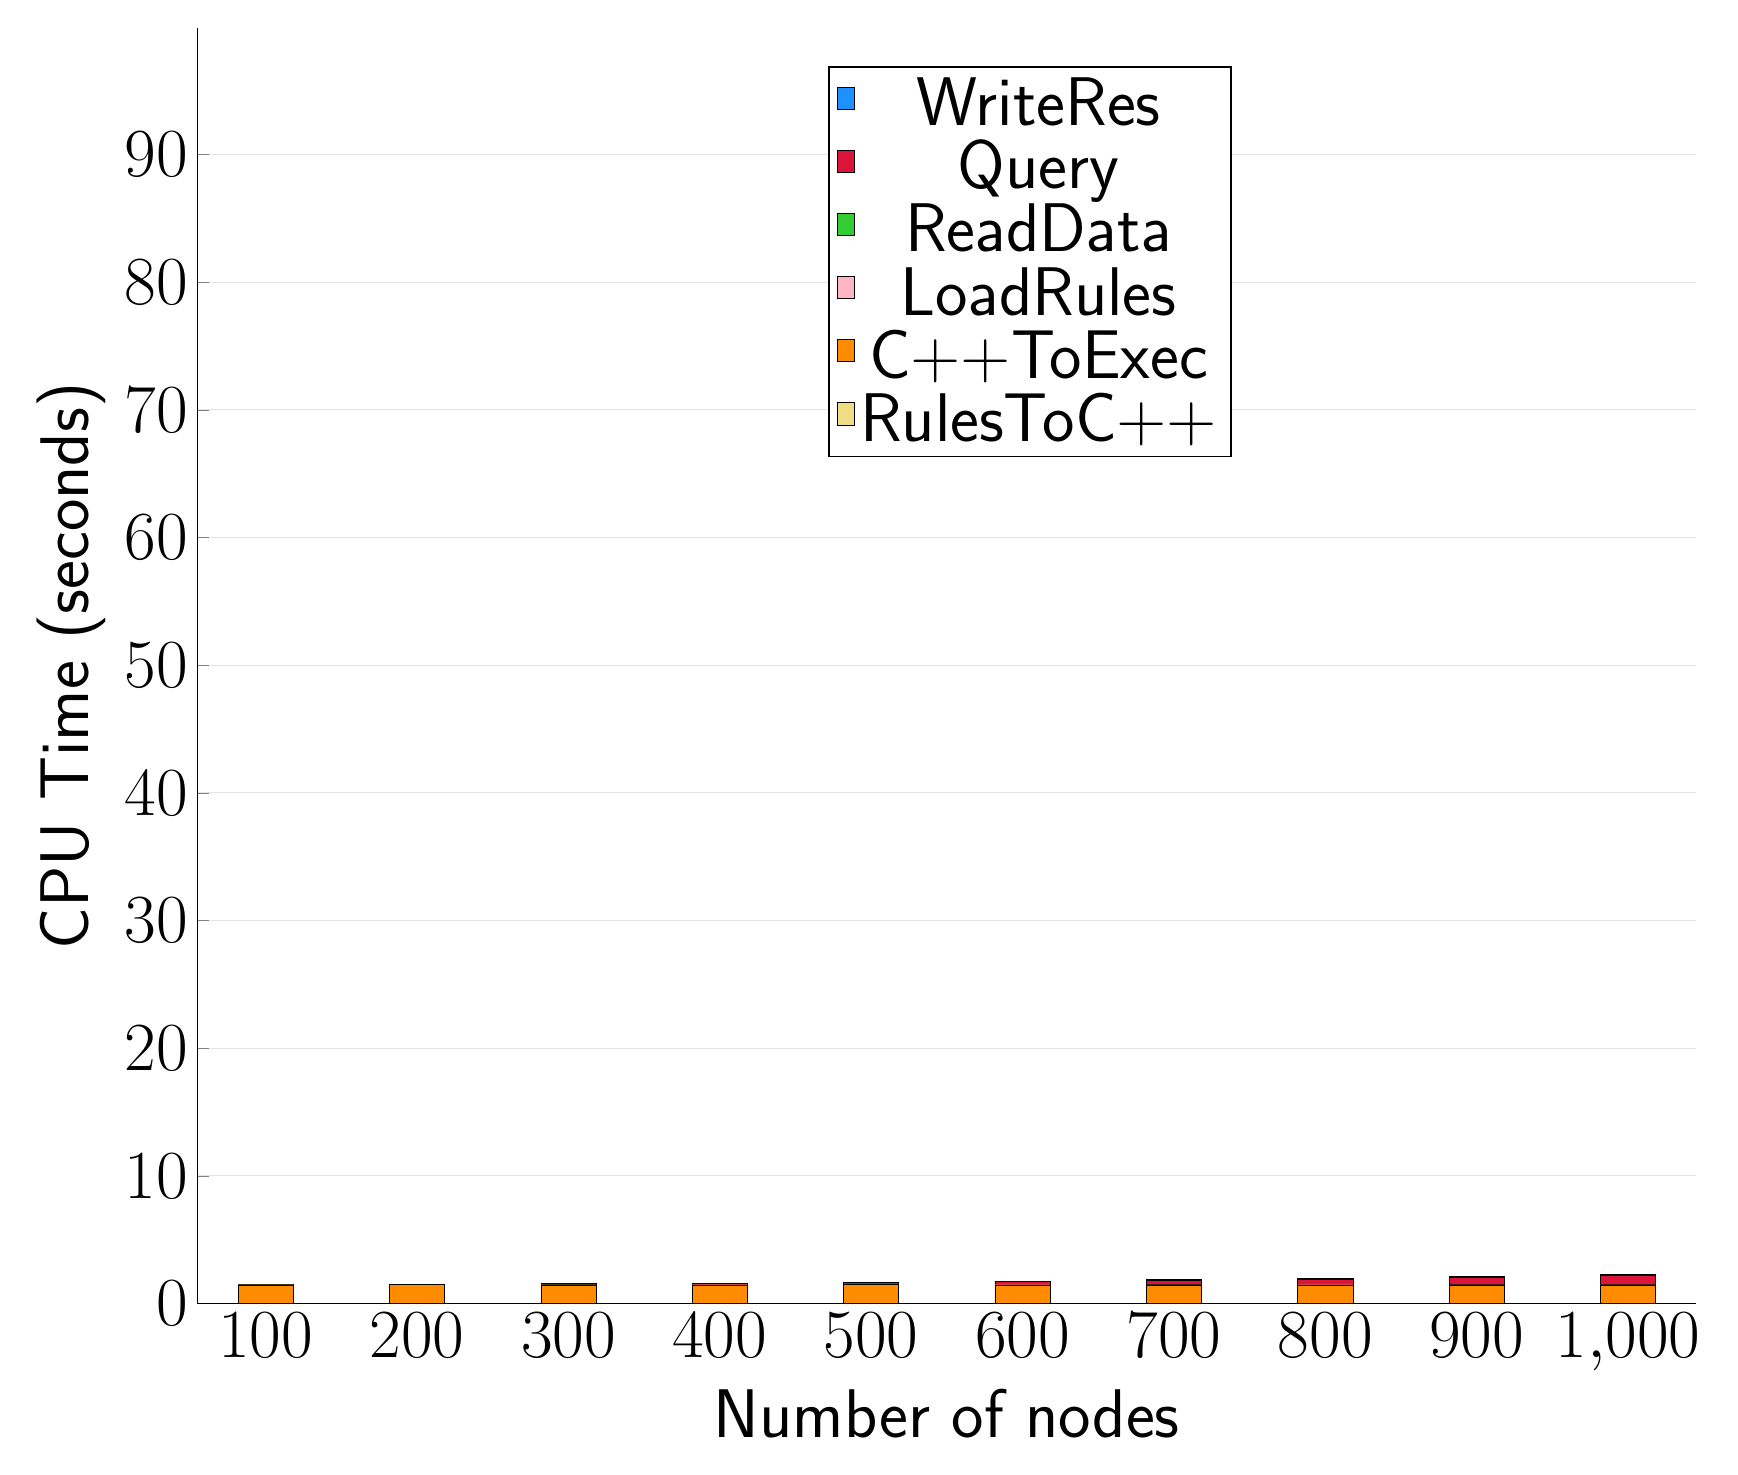
\begin{tikzpicture}
\begin{axis}[
   ybar stacked,
   width=1.7\textwidth,
   bar width=0.7cm,
   ymajorgrids, tick align=inside,
   major grid style={draw=gray!20},
   xtick=data,
   ymin=0, ymax=99.8926,
   axis x line*=bottom,
   axis y line*=left,
   enlarge x limits=0.05,
   legend style={
       at={(0.69, 0.97)},
       anchor=north east,
       legend columns=1,
       font=\Huge,
   },
   ylabel={CPU Time (seconds)},
   xlabel={Number of nodes},
   label style={font=\Huge},
   tick label style={font=\Huge},
]
\addlegendimage{fill=DodgerBlue, draw=black, line width=0.2pt}
\addlegendentry{WriteRes}
\addlegendimage{fill=Crimson, draw=black, line width=0.2pt}
\addlegendentry{Query}
\addlegendimage{fill=LimeGreen, draw=black, line width=0.2pt}
\addlegendentry{ReadData}
\addlegendimage{fill=LightPink, draw=black, line width=0.2pt}
\addlegendentry{LoadRules}
\addlegendimage{fill=DarkOrange, draw=black, line width=0.2pt}
\addlegendentry{C++ToExec}
\addlegendimage{fill=LightGoldenrod, draw=black, line width=0.2pt}
\addlegendentry{RulesToC++}
\addplot +[fill=LightGoldenrod, draw=black, line width=0.2pt] coordinates {
(100, 0.0020000000000000005)
(200, 0.010000000000000002)
(300, 0.006000000000000001)
(400, 0.0020000000000000005)
(500, 0.008000000000000002)
(600, 0.006000000000000001)
(700, 0.008000000000000002)
(800, 0.006000000000000001)
(900, 0.006000000000000001)
(1000, 0.0)
};
\addplot +[fill=DarkOrange, draw=black, line width=0.2pt] coordinates {
(100, 1.468)
(200, 1.464)
(300, 1.466)
(400, 1.466)
(500, 1.472)
(600, 1.464)
(700, 1.464)
(800, 1.462)
(900, 1.464)
(1000, 1.472)
};
\addplot +[fill=LightPink, draw=black, line width=0.2pt] coordinates {
(100, 0.0001516)
(200, 0.0001504)
(300, 0.0001518)
(400, 0.0001672)
(500, 0.000149)
(600, 0.0001544)
(700, 0.000153)
(800, 0.0001474)
(900, 0.00016219999999999999)
(1000, 0.0001602)
};
\addplot +[fill=LimeGreen, draw=black, line width=0.2pt] coordinates {
(100, 0.0009021999999999999)
(200, 0.0012797999999999998)
(300, 0.0017138000000000001)
(400, 0.0018856)
(500, 0.0023184)
(600, 0.0026596000000000002)
(700, 0.0031200000000000004)
(800, 0.0034156)
(900, 0.0038294)
(1000, 0.0043748)
};
\addplot +[fill=Crimson, draw=black, line width=0.2pt] coordinates {
(100, 0.0137654)
(200, 0.042230000000000004)
(300, 0.0782196)
(400, 0.12041539999999999)
(500, 0.18126119999999998)
(600, 0.2559458)
(700, 0.3446002)
(800, 0.44887560000000004)
(900, 0.5677639999999999)
(1000, 0.7062354)
};
\addplot +[fill=DodgerBlue, draw=black, line width=0.2pt] coordinates {
(100, 0.0025544)
(200, 0.0058687999999999995)
(300, 0.0099484)
(400, 0.0172828)
(500, 0.0267668)
(600, 0.038532)
(700, 0.05272980000000001)
(800, 0.0690892)
(900, 0.086214)
(1000, 0.1071094)
};
\end{axis}
\end{tikzpicture}

\end{document}
